\chapter{Full Case Study in English Diachrony}\label{ch:diachron}
\section{Introduction}
This chapter applies the analysis presented in the previous three chapters to a large scale case study, namely diachronic development in recipient ditransitive syntax in the history of English. As discussed in the introduction, quantitative (and especially) diachronic studies can provide a useful independent verification of analyses developed on the basis of acceptability judgements. Crucially, data from language production can provide independent verification of theories developed primarily from language comprehension (i.e., acceptability judgements).

The problem of finding empirical validation of theoretical claims is made acute by the nature of the types of claims made in theoretical linguistics. Building on the work starting during the cognitive revolution in the 50s and 60s, the goal of generative linguistics has been to study the linguistic competence of speakers, which consists of the language specific information that is needed to use a language natively (CITATIONS). As will be shown below, this linguistic competence can be separated into grammatical and non-grammatical competences. Grammaticality reflects the ability of a grammar to associate a particular utterance with a particular meaning. However, given the rampant ambiguity in natural language, the grammar of natural languages often associates multiple utterances with a particular meaning (and multiple meanings with a particular utterance). An equally crucial aspect of being a native speaker of a language is knowing which of the options produced by the grammar to use in any particular circumstance. These choices are often impacted by language specific implementations of general social or psychological factors (CITATIONS). Unfortunately, it has been known since the beginning of this enterprise that there is no direct evidence of this knowledge (CITATION), which is typical of knowledge and psychological constructs. Instead, it has been necessary to deduce the nature of the linguistic knowledge by studying its effects on language performance (see CITATIONS-FROM-PHILLIPS-LAB for discussion of the fundamentally performative aspect of linguistic data).

One of the most prominent types of linguistic performance to be used in theoretical linguistics is the acceptability judgement. These judgements reflect a native speakers sensation of naturalness/unnaturalness upon encountering a particular linguistic utterance. These sensations have a cognitive reality similar to that of pain sensations (CITATIONS). A major advantage to the acceptability judgement is that even utterances that would never occur in natural production (due to the combination of factors each of which is extremely infrequent) can still be studied. However, as mentioned in the first chapter, grammaticality is only one aspect that contributes to the sensation of naturalness; other factors such as pragmatic concerns can often render a perfectly grammatical utterance unnatural (e.g., because there is a more concise grammatical way of conveying the same information). Trained linguists (and ideal native language informants) are able to minimise contextual factors that impact naturalness by attempting to evaluate the utterance in a number of hypothetical linguistic contexts, but these techniques cannot rescue a grammatical utterance that is ruled out because of universal, overwhelming problems. These non-grammatical problems often have a gradual impact on acceptability, reflect a gradient notion of pragmatic infelicity or psychological complexity (CITATIONS).

Quantitative studies of language performance is useful for isolating these gradient factors, so that they can be factored out when studying grammaticality using performance data. Since corpora (ideally) provide multiple instances of the relevant features in a variety of pragmatic contexts, the gradient effects of non-grammatical factors can be investigated for the observed contexts and statistically extrapolated to unobserved contexts. In addition, corpora provide a means of studying diachronic processes that cannot be studied using traditional acceptability judgements, since the earlier speakers in the diachronic process are unavailable for consultation. Assuming that language change cannot radically alter the underlying grammar (since the speakers of the new variety must participate in a speech community with speakers of the old variety), it is possible to provide independent evidence of the internal structure of the relevant grammatical processes.

This chapter will begin by reviewing the analyses from the previous three chapters and discussing the diachronic implication of these analyses. This will be followed by looking at three independent changes in the history of English. The first change is the change in recipient marking, ranging from synthetic dative case in Old English to the current distribution of `to' in modern American English. The second change reflects changes in the non-grammatical competence of speakers vis-a-vis active word orders in the history of English (i.e., when does the recipient occur before the theme and vis-a-versa). Finally, the fall and rise of recipient passivisation will be examined going from Old English to modern American English.

\section{Theoretical Issues}
	Since this dissertation argues that all languages have the same underlying configuration of recipient and theme (i.e., the recipient is introduced as a dative PP in the specifier of an applicative phrase), I predict that there should be no diachronic development in base generation. However, there are a number of transformations that can apply to the base generated order and different stages of the language can vary as to which operations are grammatical and when they should apply.
	One of the major factors that impact the surface realisation of recipients is allomorphy with respect to the morphological realisation of the dative P-head. The P-head itself can receive a null realisation or be spelled out overtly (e.g., as the preposition `to'). It can also trigger concord on its complement, which causes the realisation of synthetic dative case on elements in the noun phrase. As an instance of allomorphy, these variants can be sensitive to contextual information (e.g., the properties of surrounding elements). The nature of these links are the essence of Sassurian arbitrariness and are thus predicted to be subject to drift over centuries of language change.
	In addition to morphological variation, there are a number of syntactic operations that impact both the surface order of elements and their syntactic hierarchy. Since all of these operations are optional, any stage of the language could fail to have them. Thus, grammatical change is predicted to involve gaining or loosing one of the operations. These operations are one of the main sources of ambiguity that necessitates the non-grammatical component of language competence. Thus, change could also impact the rate at which these grammatical operations apply. VP-internal scrambling derives a theme--recipient order from the underlying recipient--theme order by moving the theme to a higher specifier of the applicative phrase. Cliticisation moves a pronominal element from being an independent syntactic head to being adjoined to a head in the verbal spine (here the head will always be little-v/voice). Finally, P-incorporation can move the dative P-head out of the PP and adjoin it to the next highest head. This renders the complement of the preposition a bare DP, which makes it eligible for receiving structural case.
	Looking at passivisation, the availability and probability of the transformations discussed in the previous chapter alters the availability of the theme and the recipient to raise to subject position and receive nominative case. In addition, languages vary as to the permissability of T in assigning subject properties. The main variation is in the treatment of PPs in the search for a subject. The assignment of nominative case (as a structural case) is restricted to DPs, a fact which does not vary diachronically (modulo the presence/absence of P-incorporation). However, the search for an argument to raise to subject position shows a variety of possible treatments for PPs. PPs can be valid targets for subject raising (oblique subjects), they can be invisible for subject raising (triggering direct theme passivisation), or they can be defective interveners (requiring one of the operations from the previous paragraph to create a non-intervening configuration).
	In the history of English, almost all of the changes discussed above occur. The realisation of dative P shifts from synthetic dative case to `to' alternating contextually with a null realisation. While VP-internal scrambling is grammatical in all stages of English, the conditioning factors change moving from Old English to modern American English. Cliticisation is lost during the history of American English, while P-incorporation becomes common place. Finally, all of the possible treatments of PPs in passivisation are attested (oblique subject, direct theme passivisation and defective intervention). Crucially, in every case of a change in grammaticality, the analyses presented here can account for the surface change by positing the gain/loss of a single syntactic operation.
\section{Recipient Marking}
	Old English had synthetic dative case marking inherited from proto-Germanic. While there was a great deal of syncretism in the Old English case system \citep{Allen.1999}, there was a reliable distinction between accusative and dative case for many noun classes and in pronouns.

	By the end of the Old English period (11th century), these distinctions were breaking down. Nominal case marking was no longer reliable. While both accusative and dative pronominal forms were still being used, the forms were no longer consistently distributed along the accusative/dative case distinctions (i.e., old dative case forms would be used where previously accusative case was required and vis-a-versa). Around this time, `to' began to be used for the first time to introduce recipients. In Old English, `to' had previously been restricted to goals and addressees, i.e., the indirect object of verbs of communication \citep{Allen.1999,McFadden.2002,OED.2013}. 

	\begin{figure}[p!]
		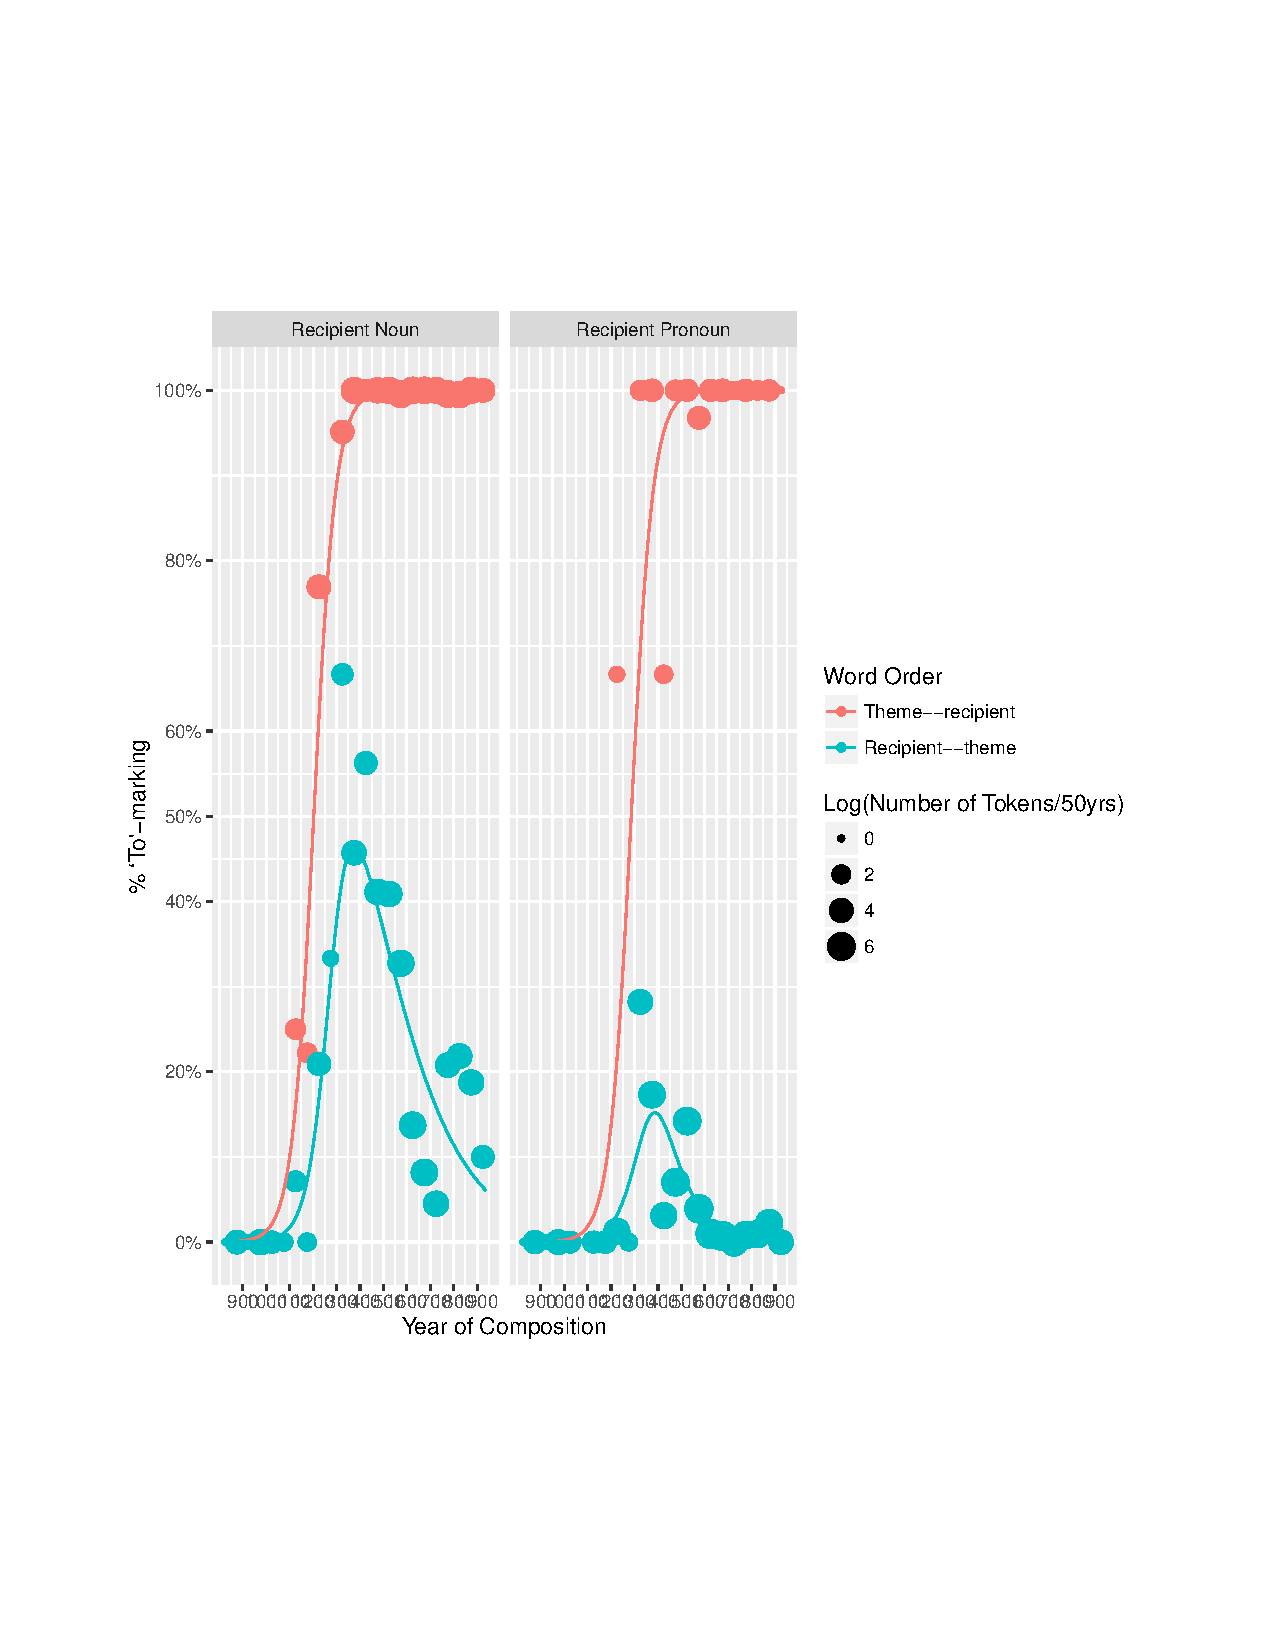
\includegraphics[width=.95\linewidth]{../images/to-marking-graph}
		\caption{Empirical frequency of `to'-use with predicted rates according to model in different conditions}
		\label{fig:to-use}
	\end{figure}

	Throughout the Middle English period (i.e., up until about 1400), `to' became more prominent across the board. However, during the 15th and 16th centuries, a new grammar arose in which the unmarked form was preferred when the recipient was adjacent to the verb. This adjacency could be satisfied either by (a) having the recipient--theme word order (e.g., ``John gave Mary the book'') or (b) by having a theme pronoun cliticise in the theme--recipient order (e.g., ``John gave it him''). In the rest of this section, I discuss statistical evidence supporting the explanation given above.

	One of the major discoveries coming from the quantitative study of diachronic syntax has been the Constant Rate Effect. This effect has obtained in cases where a single syntactic mechanism can apply in multiple syntactic environments. In these cases, it has been repeatedly found that the slope parameter assigned by logistic regression (i.e., the rate at which the frequency of use of the incoming variant changes) is constant across its different environments of application (this is true even in cases where the environments themselves show different frequencies of use). 

	The first example of this from \cite{Kroch.1989}, where the use of do-support was studied in a number of different environments (e.g., negative declaratives, affirmative questions, negative questions, imperatives, etc.). Kroch found that while the use frequency of do-support in these environments differed from one another in any given year (see Fig. \ref{fig:kroch-graph}), the rate at which these frequencies changed was constant across environments. He hypothesised that this effect reflected the fact that only one change was taking place (the loss of V-to-T raising). Under this hypothesis, the Constant Rate Effect provides a means of recovering underlying grammatical information from diachronic patterns in language use. If a Constant Rate Effect is found (assuming that one has enough data that it would be possible to fail to find it), the most parsimonious hypothesis is that there is a unified change underlying the variation in each environment.

	\begin{figure}[ht!]
		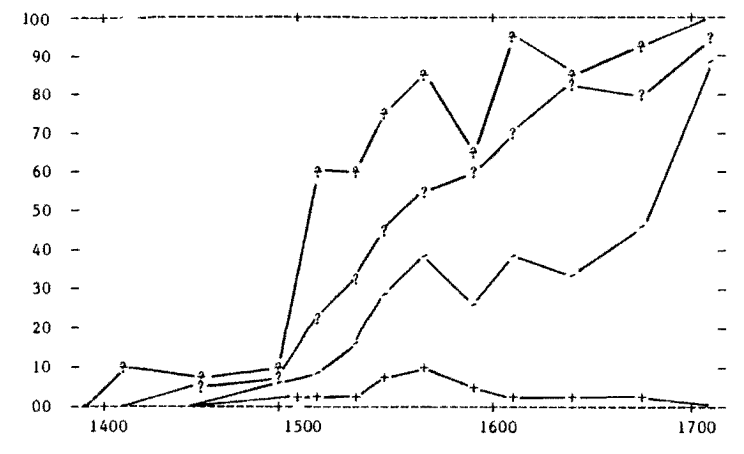
\includegraphics[width=.5\linewidth]{../images/kroch-graph}
		\caption{Rates of do-support in different environments: affirmative and negative questions (? and \sout{?}) and affirmative and negative declaratives (+ and ') (Fig. 1 from \citealt{Kroch.1989}}
		\label{fig:kroch-graph}
	\end{figure}

	For English `to'-use, there are two changes to be considered. The first is the introduction of `to' as a means of marking recipients. The second is the introduction of null marking in verb-adjacent contexts. In order to study these changes, I extracted all tokens from the Parsed Corpora of Historical English (CITATIONS) containing the following recipient introducing verbs (verbs that also introduce goals, e.g., SEND, were excluded): ALLOT, APPOINT, ASSIGN, AYEVEN, BEHIEGHT, BEQUEATH, BETAKE, DAELAN, FEED, GIVE, GRANT, LEND, OFFER, OWE, PAY, PROFFER, PROMISE, RESTORE, SELL, SELLAN, SERVE, SHOW, VOUCHSAFE, and YIELD. I also extracted information about whether the arguments were full noun phrases or pronouns, the relative order of the recipient and theme (and their order with respect to the verb to rule out cases of topicalisation), and whether or not the recipient was marked with `to' (passive data was also collected, which is discussed in the subsection below). When the theme is a pronoun, the theme--pronoun order was essentially categorical (X examples of recipient--theme order over 1000 years). Since there was such poor evidence for the frequency of `to'-use in these environments, their inclusion muddled any attempts at statistical analysis. Therefore, those cases have been excluded for the analyses discussed below (and were excluded from Fig. \ref{fig:to-use} as well).

	As can be seen in Fig. \ref{fig:to-use}, in theme--recipient contexts, the frequency of `to' use increased in the typical S-shaped curve expected from logistic regression \citep{Kroch.1989}. However, when both the recipient and theme were a pronoun, the S-shaped curve did not go to 100\%, reflecting the availability of theme pronoun cliticisation to render the null allomorph available. This effect was captured in the models by scaling the logistic. The scaling was accomplished by multiplying the outcome of the logistic by a scaling factor. This scaling factor was derived from an independent logistic regression (guaranteeing that the scaling factor would be between 0 and 1), which allowed the both pronoun case to differ in scale from all the other environments.

	The same scaling issues arise in the recipient--theme orders. Even after the null allomorphy grammar has taken hold, `to' still occurs in recipient--theme orders because of heavy NP shift (e.g., ``John gave to me the book that he wrote last summer.'). The same mechanism that captures this scaling was also able to capture the fact that the null allomoprhy change only affected the recipient--theme orders (i.e., by scaling the effect of the change to 0 in the theme--recipient environments). This interaction of changes do not show a typical S-shaped curve. Instead, as discussed above, `to'-use until about 1400 and then slowly tapers off. As discussed in \cite{Bacovcin.2016}, this effect can be modelled by multiplying two independent logistic changes together. An advantage of separating the change into two distinct logistics, is that the Constant Rate Effect can be tested for. In other words, it was possible to see if the rise of `to' in theme--recipient and recipient--theme contexts reflected a uniform underlying change. The Constant Rate Effect predicts the \textbf{absence} of significant interactions between year and condition factors (in this case, word order and the status of the theme and recipient). 

	The final model involved the multiplication of four distinct logistic regressions. Two of the regressions were used to calculate the scaling parameters (one for each change), and the other two represented the changes themselves. The general structure of logistic regression is: 1/(1+exp(-parameters)), where the parameters are a linear model (i.e. predicting a number ranging from -Inf to +Inf) that is transformed into a number between 0 and 1. The final model for all environments discussed here was: (1/(1+exp(-(change1scaling))))*(1/(1+exp(-(change1parameters))))*(1-((1/(1+exp(-(change2scaling))))*(1/(1+exp(-(change2parameters)))))). The interpretation of this is that the first two logistic equations generated a scaled implementation of the rise of `to'-use, while the second two equations generated a scaled version of the rise of the null allomorphy grammar. The results of the null allomorphy grammar were subtracted from 1 so that when multiplied with the first change, there would be little effect early on and then a larger effect later. Also, this allowed the scaling in the theme--recipient environment to go to zero and have no effect on the first change. This complex model was fit using the nloptr R package for non-linear optimisation (see the accompanying R files for more detail). The optimum model was found using stepwise AIC, where parameters were individually added to the model (always including the parameter that created the greatest decrease in AIC) until no further improvement was found.

	The optimal model had the following properties (model fits shown in Fig. \ref{fig:to-use}): (a) the first change was characterised by a slope parameter, a scaling parameter when both arguments were pronouns, and a basic effect when both arguments were pronouns, (b) the second change was characterised by a slope only for recipient--theme orders, a constant effect of recipient pronouns, and a scaling factor that varied between word orders. Effect (a) indicates an extremely strong Constant Rate Effect for the introduction of `to'-marking for recipients, there was no significant variation across conditions. Part of that is because variation was captured by the second change (the null allomorphy change). This change had a constant effect of depressing `to'-marking with recipient pronouns (similar to the effect in Romance languages, where clitic pronouns receive null marking while full noun phrases receive prepositional marking). The interaction of a scaling parameter and the constant pronominal effect generated the lower end point for the theme--recipient orders when both objects were pronouns. In the recipient--theme order, it also had an effect of decreasing `to'-use over time as the null allomorph in adjacent contexts grammar spread through the population.

	This modelling technique allowed for confirmation of another case of the Constant Rate Effect, involving a complex interaction of properties. Data from the corpus on the spread of `to'-marking is strongly consistent with it involving a single change across all recipient constructions. The complex allomorphy seen in Modern British English can be explained as the interaction of this simple morphological change in the base realisation of recipient marking in combination with two additional morphological operations. The first is a time independent dispreference for marking recipient pronouns with overt case markers (a fact that may be linked to the maintenance of a synthetic case distinction on pronouns). The other is the introduction of the adjacency trigger null allomorphy, which becomes prominent during the 15th and 16th centuries.

\section{Passivisation Order}
	Changes in passivisation of ditransitives is a more complex change. The situation in Old English is quite complex. \cite{Allen.1999} provides evidence that monotransitive datives are able to become oblique subjects in Old English, but she suggests that in ditransitives, putative oblique subjects are actually topics. To discuss this distinciton, she introduces the term ``fronted dative'', which is agnostic as to whether the fronted element is a topic or a subject. The argument about the status of fronted datives in ditransitive passives is made on the basis of Coordinate Subject Deletion facts.
	In Old English (as in Modern English), arguments are generally obligatory (i.e., neither subject nor object drop is licensed). However, when two sentences are coordinated and share the same subject, the subject does not need to be expressed in the second sentence (\ref{ex:OECSD}). In a corpus investigation, none of the fronted datives in ditransitive passives triggered Coordinate Subject Deletion, while a number of fronted nominatives did (see Table \ref{tab:AllenOECSD}). 

	\begin{table}
		\begin{tabular}{cccc}
			Nominative Coreferential & & Deletion & No Deletion \\
			& Order NOM DAT & 11 & 4 \\
			& Order DAT NOM & 4 & 3 \\
			& Total & 15 & 7 \\
			Dative Coreferential & & Deletion & No Deletion \\
			& Order NOM DAT & 0 & 27 \\
			& Order DAT NOM & 0 & 11 \\
			& Total & 0 & 38 \\
		\end{tabular}
		\caption{Allen's counts of Coordinate Subject Deletion with ditransitive passive in OE prose (Table 2-6, \citealt{Allen.1999})}
		\label{tab:AllenOECSD}
	\end{table}

	\begin{exe}
		\ex \label{ex:OECSD} \gll ða easternan tungelwitegan gesawon niwne sterorran beorhtne, na on heofnum betwux oðrum tunglum, \textbf{ac} \textbf{w\ae s} angenga betwux heogenum and eorðan\\
		the eastern star-wisemen saw new.ACC star.ACC bright.ACC, not in heaven among other stars, \textbf{but} \textbf{was} solitary between heaven and earth\\
		\trans `The eastern star-wisemen saw a bright, new star, not in the heaven among other stars, but it was solitary between heaven and earth (Ex. 29, \citealt{Allen.1999}).'
	\end{exe}

	There are two problems with this argument. In the first case, the total number of coordinated passive sentences is not very large, so it is possible that the lack of dative examples is merely accidental. This is made even more serious because of Standard German facts. While Standard German is generally accepted to not have oblique subjects (\citealt{Zaenen.1985}, although see \citealt{Eythorsson.2005}), it does allow fronted dative elements to trigger coordinate topic deletion, but only if the two topic share the same case (CITATIONS). Assuming that Old English had the same rules, (a) Coordinate Subject Deletion would need to be distinguished from Coordinate Topic Deletion and (b) the fact that fronted dative elements are rarer than fronted nominative elements would need to be accounted for before any data was interpreted. 
	In additions to the problems with her argument discussed above, I have data from the Corpus of Old English Prose \citep{Taylor.2003} that suggests that fronted datives in Old English ditransitive passives were actually subjects. In Old English, the status of the theme and recipient as noun vs pronoun had a nearly categorical effect on active word order, with recipient pronouns coming before theme nouns and theme pronouns coming before recipient nouns and pronouns. The exact same ordering sensitivity is found for the fronted element in the passive, which can be explained if these fronted elements are subjects (oblique or otherwise) and the highest element in the active raises to subject in the passive. If they were topics, it is unclear why topicality should be sensitive to active word order in this way.

	INSERT TABLE HERE
	
	This match between active and passive orders ceases after the Old English period. The move from Old English to Modern English is characterised by the loss of recipient fronting. Much of this loss occurs during the 11th and 12th centuries (where our data is sparsest), however, by the 13th century, ditransitives with initial recipients are quite uncommon (see Fig. X). This loss of recipient fronting begins as a loss of oblique subjects. However, by at least 1375, dative--to--nominative conversion had become a live possibility \citep{Allen.1999}. Interestingly, this change in the origins of recipient subjects in passives (from oblique subjects to dative--to--nominative conversion) did not prevent (or seemingly alter) the loss of recipient passivisation.

	INCLUDE PROOF OF CONTINUITY

	INSERT FIGURE OF RECIPIENT PASSIVISATION

	Under the system proposed here, this change reflects a move away from having either PP passives or P-incorporation. Together these reflect a dispreference for manipulating PPs. If the PP cannot move to subject position or be incorporated, then theme passivisation becomes obligatory. While P-incorporation is grammatical (as can be seen by the existence of pseudo-passives and the occasional instance of dative--to--nominative conversion), it is strongly dispreferred, apparently because any such manipulation of PPs was dispreferred. This reflects a case where the grammar can generate possibilities that are selected against. In other words, for pseudo-passives P-incorporation is the only possible way of demoting the agent (assuming this is the main pragmatic role of passivisation). However, for ditransitives, P-incorporation is only one of a set of possible operations that license ditransitive passivisation. Building on previous generations loss of oblique subjects, there was a dispreference for manipulating PPs, which extended to the use of P-incorporation when other options were available.

	This separation of active and passive word orders continues in British English to the end of our data (in abt. 1911). However, the change is reversed in American English. Looking at data from the Corpus of Historical American English \citep{Davies.2010}, I extracted all instances of passive sentences involving the verbs `give' or `offer'. For `give', I hand coded all of the examples, while for offer I coded a sample of X tokens for each year. Each token was coded for the type of passive (theme, recipient, or monotransitive), the status of the recipient (full noun phrase or pronoun), and the marking of the recipient (presence/absence of `to'). For `offer', I also hand coded the status of the theme (full noun phrase or pronoun). For `give', I use a script to determine where the theme was (based on the type of passive coding) and then determined the status of the theme automatically.
	
	The result of this study shows that the main change in ditransitive passives in American English was an increase in the rate of recipient passivisation. In the early 19th century, there are essentially no examples of recipient passives. By the end of the 20th century, recipient passivisation rates match active word order rates (see Fig. X). Logistic regression models confirm that the change in recipient passivisation during this period is significant (INSERT STATS HERE). Just as in Old English, ditransitive passive word order reflected active ditransitive word order.

	INSERT TABLE COMPARING ACTIVE AND PASSIVE WORD ORDERS IN LATE 20th CENTURY AMERICAN ENGLISH

	According to the analyses proposed here, this change in American English reflects a normalisation of P-incorporation. In Early Modern English (and at least early 20th century British English), P-incorporation was a marked operation. If there was no other way of implementing passivisation (i.e., in the case of pseudo-passivisation), P-incorporation was available. However, if possible, speakers preferred to use other mechanisms for licensing passivisation. In American English, however, P-incorporation became a normal state of affairs. Given that the preposition is realised as $\emptyset$ in recipient--theme orders, there is no surface evidence against P-incorporation. Therefore, language learners only have indirect evidence for the rate of P-incorporation; this reliance on indirect evidence creates a situation that is ripe for language change.

\section{Conclusions}
	In this chapter, I have presented two case studies of change in the history of English. The first captured changes in morphological marking of recipients, which supports the interchangeability of prepositional and synthetic case marking. The second the fall and rise of recipient passivisation. The first change provided an example of how even complex changes involving the interaction of a number of moving parts (two changes each of which involved scaling factors) can be broken apart using relatively simple statistical processes. This breaking apart can then provide evidence for the structure of the underlying grammar. The second change provided some insight into the underlying mechanism driving changes in use frequency of syntactic mechanisms. In at least some cases, it is the surface outcome of the mechanisms that is subject to change (i.e., recipient passives), independently of how that surface property is derived (i.e., oblique subjects vs. dative-to-nominative raising). While in many cases the surface properties that drive use-frequency changes are the direct reflexes of grammatical properties (as was the case with changes in allomorphy in the `to'-marking change), in other cases the relationship between use and grammar is more indirect with surface properties that have multiple grammatical causes being unified by language learners.

%\bibliography{diss}
